\chapter{Ứng dụng ngôn ngữ Rust}
\section{Chọn vi xử lý để thực hiện lập trình nhúng trong Rust}
Trước khi thực hiện lập trình nhúng cho bất kỳ hệ thống nào, ta phải chọn một vi điều khiển phù hợp cho hệ thống đó trước.

Trước hết, tôi đưa ra một số vi xử lý thông dụng, phù hợp, được sử dụng để giảng dạy về lập trình hệ nhúng ở trường Đại học Bách Khoa TP.HCM, so sánh chúng và từ đó chọn một vi xử lý phù hợp với nhu cầu.
\subsection{Một số vi xử lý thông dụng}
\subsubsection{MSP-EXP430G2 Evaluation board}
\begin{figure}[ht]
\centering
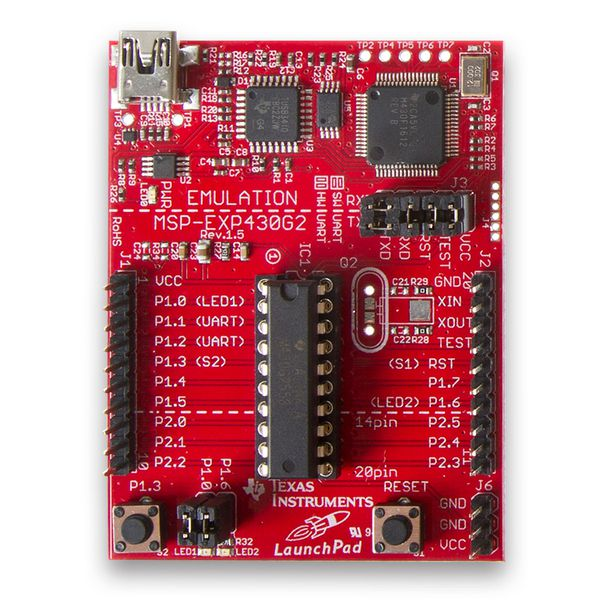
\includegraphics[scale=0.35]{images/launchpad-mspexp430g2-02.jpg}
\caption{MSP-EXP430G2}
\end{figure}
\clearpage

MSP-EXP430G2 \cite{msp430_datasheet} (hay MSP430) là dòng vi điều khiển của Texas Instrument (TI), 16 bit, kiến trúc RISC được thiết kế đặc biệt cho siêu năng lượng thấp.

\textbf{Một số hiệu năng nổi bật của MSP430}
\begin{itemize}
    \item CPU 16 bit tốc độ \si{16\MHz}.
    \item 16 KB Flash.
    \item 512B SRAM.
\end{itemize}

\textbf{Ưu điểm}: Giá thành rẻ, nhỏ gọn, đầy đủ các ngoại vi thông dụng. Có bộ thư viện phong phú dễ dàng thực hiện lập trình nhúng trên nhiều lĩnh vực.

\textbf{Nhược điểm}: Khá ít bộ nhớ SRAM, cũng như tốc độ CPU còn hạn chế, và CPU chỉ hỗ trợ tính toán 16 bit nên sẽ khó có thể thực hiện tính toán nặng trên MSP430.

\subsubsection{STM32F103C8T6 - Blue Pill}
\begin{figure}[ht]
\centering
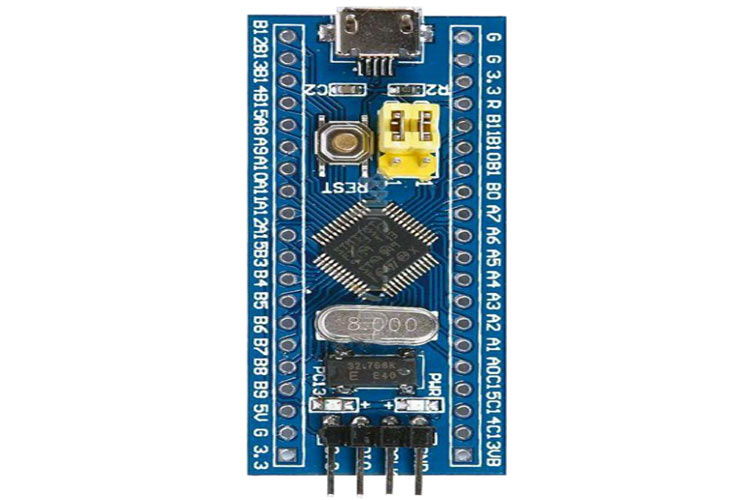
\includegraphics[scale=0.35]{images/STM32-Blue-Pill-Development-Board.jpg}
\caption{STM32 Blue Pill}
\end{figure}
STM32F103C8T6 \cite{blue_pill_datasheet} (hay Blue Pill) là một vi xử lý rất thông dụng của ST-Microelectronics, sử dụng CPU Arm-Cortex M3, 32 bit với giá thành rẻ.

\textbf{Một số hiệu năng nổi bật của Blue Pill}
\begin{itemize}
    \item CPU ARM-Cortex M3 32 bit tốc độ \si{72\MHz}, 1.25 DMIPS/MHz.
    \item 128 KB Flash.
    \item 20 KB SRAM.
\end{itemize}

\textbf{Ưu điểm}: Giá thành rẻ, nhỏ gọn, đầy đủ các ngoại vi thông dụng. CPU mạnh mẽ. Kèm theo một số ngoại vi khác như RTC.

\textbf{Nhược điểm}: Vì Blue Pill sử dụng CPU ARM-Cortex M3 nên một số tính năng tính toán nặng như DSP sẽ không được phần cứng hỗ trợ. Ngoài ra, ta không thể flash trực tiếp chương trình lên Blue Pill được mà phải thông qua một Bootloader như ST-Link/V2 \cite{stlinkv2_datasheet}.

\subsubsection{Arduino Uno R3}
\begin{figure}[ht]
\centering
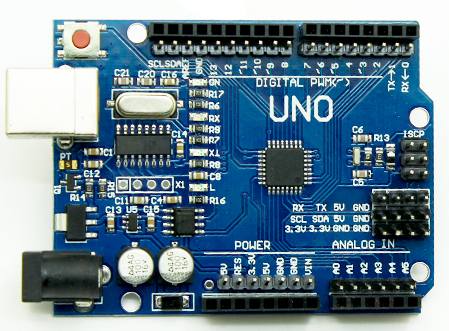
\includegraphics[scale=0.75]{images/Arduino-Uno-R3-SMD.jpg}
\caption{Arduino Uno R3}
\end{figure}

Arduino Uno R3 \cite{arduino_datasheet} là loại phổ biến và dễ sử dụng nhất trong các dòng Arduino hiện nay cũng như tương thích với nhiều Arduino Shield.

\textbf{Một số hiệu năng nổi bật của Arduino Uno R3}
\begin{itemize}
    \item CPU ATmega328P 8 bit tốc độ \si{16\MHz}.
    \item 32 KB Flash.
    \item 1 KB EEPROM.
    \item 2 KB SRAM.
\end{itemize}

\textbf{Ưu điểm}: Giá thành rẻ, nhỏ gọn, đầy đủ các ngoại vi thông dụng.

Có rất nhiều thư viện abstraction C/C++ chất lượng cao, dễ sử dụng.

\textbf{Nhược điểm}: Hiệu năng tính toán của Arduino Uno R3 tương đối hạn chế.

AVR \mintinline{bash}{avr-unknown-gnu-atmega328} là đối tượng bậc 3 của bộ compiler trong Rust \cite{rustc_book}, vì vậy lập trình trên vi điều khiển này sẽ gặp nhiều chướng ngại vật, khó có thể đánh giá khách quan về hệ thống.

\clearpage
\subsubsection{EK-TM4C123G}
\begin{figure}[ht]
\centering
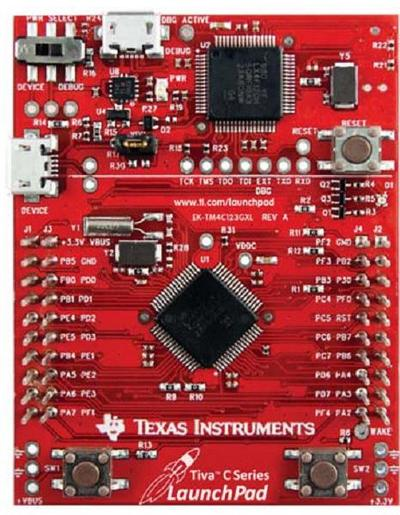
\includegraphics[scale=0.5]{images/kit_tivac.jpg}
\caption{Evaluation Kit EK-TM4C123G}
\end{figure}

EK-TM4C123G \cite{tivac_datasheet} (hay kit Tiva C launchpad) được phát triển bởi tập đoàn Texas Instruments để thay thế cho sản phẩm Stellaris Launchpad đã dừng sản xuất trước đó.
Dòng Tiva C 32-bit được sử dụng trong đề tài này có một thiết kế hiện đại cùng tập lệnh phong phú và hệ sinh thái về code nhúng giàu có
đã đẩy nhanh việc giảng dạy về lập trình nhúng nói chung trong môi trường trường học cũng như cũng đủ mạnh mẽ để có thể phát triển thêm lên để sử dụng trong môi trường công nghiệp hiện đại.

\textbf{Một số hiệu năng nổi bật của Tiva C launchpad}
\begin{itemize}
    \item CPU ARM-Cortex M4F 32 bit tốc độ \si{80\MHz}, 1.25 DMIPS/MHz.
    \item 256 KB Flash.
    \item 32 KB SRAM.
    \item 2 KB EEPROM.
\end{itemize}

\textbf{Ưu điểm}: Giá thành rẻ, nhỏ gọn, mạnh mẽ. Có bộ thư viện phong phú dễ dàng thực hiện lập trình nhúng trên nhiều lĩnh vực.
Khả năng hoạt động với chế độ tiết kiệm điện để hoạt động liên tục, phù hợp cho việc áp dụng cho môi trường thực tiễn.

\textbf{Nhược điểm}: Giá thành vẫn còn đắt hơn so với một số thiết bị STM32 với cùng hiệu năng. (khoảng 350000 VNĐ ở thời điểm tháng 06/2021)

\clearpage
\subsubsection{STM32F411 Discovery}
\begin{figure}[ht]
\centering
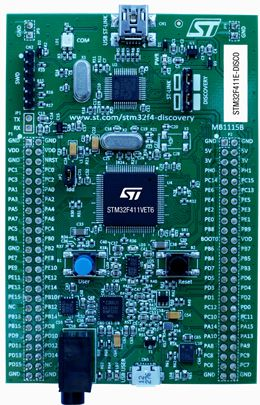
\includegraphics[scale=0.5]{images/en-stm32f411e-disco.jpg}
\caption{STM32F411 Discovery}
\end{figure}

STM32F411 \cite{discovery_datasheet} (hay STM32 Discovery) là một phiên bản nâng cấp của kit STM32F407 Discovery được sử dụng rất phổ biển hiện nay trong các nghiên cứu về dòng ARM STM32F4.
Kit có tích hợp sẵn mạch nạp ST-Link/V2, các ngoại vi như cảm biến gia tốc, từ trường, audio, v.v..

\textbf{Một số hiệu năng nổi bật của STM32 Discovery}
\begin{itemize}
    \item CPU ARM-Cortex M4 + DSP Core 32 bit tốc độ \si{100\MHz}, 1.25 DMIPS/MHz.
    \item 512 KB Flash.
    \item 128 KB SRAM.
\end{itemize}

\textbf{Ưu điểm}: Các thông số hiệu năng cực kỳ mạnh mẽ, kèm theo DSP Core cũng như tích hợp một số ngoại vi khác như cảm biến gia tốc, từ trường, audio, v.v..

\textbf{Nhược điểm}: Giá thành tương đối đắt (khoảng 500.000 VNĐ ở thời điểm tháng 06/2021).

\subsubsection{Raspberry Pi 3 Model B+}
\begin{figure}[ht]
\centering
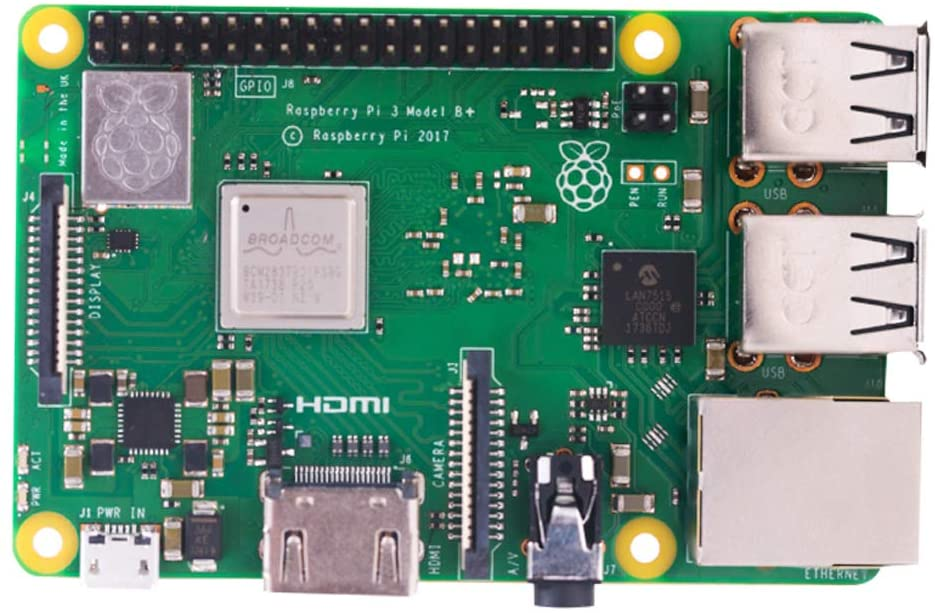
\includegraphics[scale=0.25]{images/raspberry-pi-model-3bplus.jpg}
\caption{Raspberry Pi 3 Model B+}
\end{figure}
Máy tính Raspberry Pi 3 Model B+ \cite{raspberry_datasheet} là một trong những sản phẩm tương đối mới, nổi bật với 4 nhân 64 bit CPU ARM-Cortexv8 với tốc độ lên đến 1.4 GHz.
Máy tính Raspberry Pi 3 Model B+ đủ mạnh để có thể chạy được một hệ điều hành như Linux.

\textbf{Một số hiệu năng nổi bật của Raspberry Pi 3 Model B+}
\begin{itemize}
    \item Quad-core CPU ARM-Cortex-A53 64 bit tốc độ \si{1.2\GHz}.
    \item 1 GB RAM.
    \item Đi kèm với VideoCore IV multimedia/3D graphic core.
\end{itemize}

\pagebreak
\textbf{Ưu điểm}: Có hiệu năng vượt trội hơn hẳn tất cả các vi điều khiển đã liệt kê trước.

Thư viện hỗ trợ cho Raspberry Pi có thể được xem là một trong những thư viện đầy đủ nhất.

Raspberry Pi 3 Model B+ đủ mạnh để có thể chạy hệ điều hành Linux nên ta có thể lập trình nhúng cực kỳ dễ dàng và hiệu quả.

\textbf{Nhược điểm}: Giá thành đắt. Tại thời điểm tháng 06/2021 thì giá thành của một kit Raspbery Pi 3 Model B+ là khoảng 1100000 VNĐ chưa kèm phụ kiện.

\subsection{Lựa chọn vi điều khiển}

Ở đây, để thực hiện ứng dụng Rust cho một hệ thống nhúng thực tế, tôi đưa ra một số yêu cầu để thử nghiệm ngôn ngữ này.

\begin{itemize}
    \item Vi điều khiển này có đầy đủ các chức năng của một vi điều khiển thông dụng, để ta có thể dễ dàng thử nghiệm toàn bộ những ngoại vi cơ bản.
    \item Vi điều khiển này được hỗ trợ tương đối tốt, cả trong C lẫn Rust để ta có thể dễ dàng so sánh kết quả trong quá trình thiết kế hệ thống nhúng.
    \item Vì Rust là một ngôn ngữ cấp thấp, tôi muốn thử nghiệm tính toán nặng trên vi điều khiển để kiểm tra về tốc độ của Rust trong một hệ thống thực tế.
    \item Giá thành tương đối rẻ.
        Trong lập trình nhúng, thiết kế các hệ thống với những giới hạn nhất định về phần cứng cũng như về giá thành của hệ thống là một công việc mà người thiết kế hệ thống thường xuyên gặp phải.
        Vì vậy, Rust phải hỗ trợ những vi điều khiển giá rẻ, không được giới hạn bởi các vi điều khiển cao cấp.
\end{itemize}

Dựa trên các yêu cầu này, có thể thấy có hai lựa chọn về vi xử lý để thực hiện những yêu cầu này là kit Tiva C và kit STM32 Discovery.

Ở đây, tôi quyết định chọn kit Tiva C làm đối tượng để nghiên cứu trong đề tài này vì giá thành của nó rẻ hơn so với kit STM32 Discovery.

\section{Viết phần mềm nhúng cho vi điều khiển trong Rust}
Trước khi thực hiện viết chương trình nhúng cho vi điều khiển, ta cần chuẩn bị một số công cụ để thực hiện điều này.

\begin{itemize}
    \item Các công cụ của Rust: chi tiết cài đặt có thể xem tại website chính thức Rust Programming Language \cite{rust_website}.
    \item Cargo clone: cài đặt thông qua \mintinline{bash}{cargo install cargo-clone} \cite{cargo_clone}.
    \item Một số các công cụ biên dịch mã cho đối tượng ARM:

    \mintinline{bash}{arm-none-eabi-gcc arm-none-eabi-ar arm-none-eabi-objcopy}
    \item Công cụ flash cho Tiva C: \mintinline{bash}{lm4flash} \cite{lm4tools}.
    \item GDB cho đối tượng ARM: \mintinline{bash}{gdb-arm-none-eabi} \cite{gdb_website}.
    \item OpenOCD: \mintinline{bash}{openocd} \cite{openocd_website}.
\end{itemize}

Ở đây, vì kit Tiva C có một BSP là \mintinline{bash}{stellaris-launchpad} \cite{stellaris_launchpad_bsp} nên tôi sẽ sử dụng crate này để đấy nhanh tiến độ thực hiện lập trình.

Trước hết, ta tham khảo cấu trúc của crate \mintinline{bash}{stellaris-launchpad} qua ví dụ \ref{lst:stellaris_launchpad_structure}.

\begin{listing}
\dirtree{%
.1 stellaris-launchpad/.
.2 .cargo.
.2 examples.
.2 src.
.2 .gdbinit.
.2 Cargo.lock.
.2 Cargo.toml.
.2 build.rs.
.2 memory.x.in.
}
\caption{Cấu trúc của crate BSP stellaris-launchpad}
\label{lst:stellaris_launchpad_structure}
\end{listing}

Ta thấy nó tương tự với cấu trúc một dự án Rust cơ bản (xem trang \pageref{lbl:basic_rust_proj_structure}), nhưng có thêm một số file khác.
Tôi đi tiến hành phân tích về công dụng của các file này.

\textbf{.gdbinit}

File này chứa các lệnh của GDB sẽ thực hiện khi khởi động GDB \cite{gdbinit}.

\textbf{build.rs}

Một số thư viện cần phải biên dịch thêm một số mã nguồn khác (như C), một số khác cần phải link với các thư viện C trên hệ thống hay biên dịch từ mã nguồn.

Vì \mintinline{bash}{cargo} không thể thực hiện những điều này nên file \mintinline{bash}{build.rs} được sử dụng để thông báo cho \mintinline{bash}{cargo} rằng nó sẽ không thực hiện biên dịch mã trực tiếp mà sẽ thông qua một số bước khác được định nghĩa trong file này \cite{cargo_book}.

\textbf{memory.x}

File này chứa thông số về địa chỉ FLASH và địa chỉ RAM cũng như độ lớn của chúng.

Ví dụ \ref{lst:memory_x} là nội dung file \mintinline{bash}{memory.x} của crate BSP \mintinline{bash}{stellaris-launchpad}.

\begin{listing}[ht]
\begin{plaintext}
MEMORY
{
    FLASH (rx) : ORIGIN = 0x00000000, LENGTH = 0x00040000
    RAM (rwx) : ORIGIN = 0x20000000, LENGTH = 0x00008000
}
\end{plaintext}
\caption{Một ví dụ về file memory.x}
\label{lst:memory_x}
\end{listing}

Dựa theo hướng dẫn của crate, ta thấy rằng, các dự án sẽ được viết và đặt trong thư mục \mintinline{bash}{examples}.

Biên dịch sử dụng lệnh \mintinline{bash}{cargo build --example <name> --release}.

Chuyển thành dạng binary sử dụng lệnh \mintinline{bash}{arm-none-eabi-objcopy -O binary tgt dst}

Và cuối cùng là flash file binary lên kit bằng lệnh \mintinline{bash}{lm4flash dst.bin}

Tôi tiến hành viết một số chương trình có độ khó từ đơn giản đến phức tạp để thử nghiệm Rust trên Tiva C.

\subsection{Chương trình nháy LED}
Chương trình nháy LED được xem là chương trình đơn giản nhất trong một hệ thống nhúng.
